\documentclass[10pt]{article}
\usepackage[utf8]{inputenc}
\usepackage[spanish]{babel}
\usepackage{amsmath}
\usepackage{amsfonts}
\usepackage{amssymb}
\usepackage{graphics}
\usepackage{graphicx}
\usepackage[left=2cm,right=2cm,top=2cm,bottom=2cm]{geometry}
\usepackage{imakeidx}
\makeindex[columns=3, title=Alphabetical Index, intoc]
\usepackage{listings}
\usepackage{multicol}
\usepackage{changepage}
\usepackage{float}
\usepackage{cite}
\usepackage{url}
\usepackage{hyperref}
\usepackage{pdflscape}
\usepackage[document]{ragged2e}
\usepackage{xcolor,colortbl}

\hypersetup{
    colorlinks=true,
    linkcolor=blue,
    filecolor=magenta,
    urlcolor=blue,
}

\definecolor{Red}{rgb}{0.7,0,0}
\definecolor{LightCyan}{rgb}{0.88,1,1}
\definecolor{AquaCyan}{rgb}{0.2,1,0.5}
\definecolor{Gray}{gray}{0.85}
\definecolor{DarkBlue}{rgb}{0.1,0.1,0.5}

\definecolor{codegreen}{rgb}{0,0.6,0}
\definecolor{codegray}{rgb}{0.5,0.5,0.5}
\definecolor{codepurple}{rgb}{0.58,0,0.82}
\definecolor{backcolour}{rgb}{0.95,0.95,0.92}

\lstdefinestyle{mystyle}{
    backgroundcolor=\color{backcolour},
    commentstyle=\color{codegreen},
    keywordstyle=\color{magenta},
    numberstyle=\tiny\color{codegray},
    stringstyle=\color{codepurple},
    basicstyle=\ttfamily\footnotesize,
    breakatwhitespace=false,
    breaklines=true,
    captionpos=b,
    keepspaces=true,
    numbers=left,
    numbersep=5pt,
    showspaces=false,
    showstringspaces=false,
    showtabs=false,
    tabsize=3
}
\def\fillandplacepagenumber{%
 \par\pagestyle{empty}%
 \vbox to 0pt{\vss}\vfill
 \vbox to 0pt{\baselineskip0pt
   \hbox to\linewidth{\hss}%
   \baselineskip\footskip
   \hbox to\linewidth{%
     \hfil\thepage\hfil}\vss}}
\lstset{style=mystyle}

\title{Introducción a bases de datos\\Sesión 4}

\author{Adrian González Pardo}

\date{\today}

\newcommand\tab[1][1cm]{\hspace*{#1}}

\begin{document}
\maketitle
\section{MySQL}
\subsection{Ejemplos}
\begin{center}
  \lstinputlisting[language=sql]{ejemplo1.sql}
  \lstinputlisting[language=sql]{ejemplo2.sql}
  \lstinputlisting[language=sql]{ejemplo3.sql}
\end{center}
\clearpage
\subsection{Retos}
\begin{center}
  \lstinputlisting[language=sql]{reto1.sql}
  \lstinputlisting[language=sql]{reto2.sql}
\end{center}
\clearpage
\subsection{Capturas de ejecución en servidor}
\begin{center}
  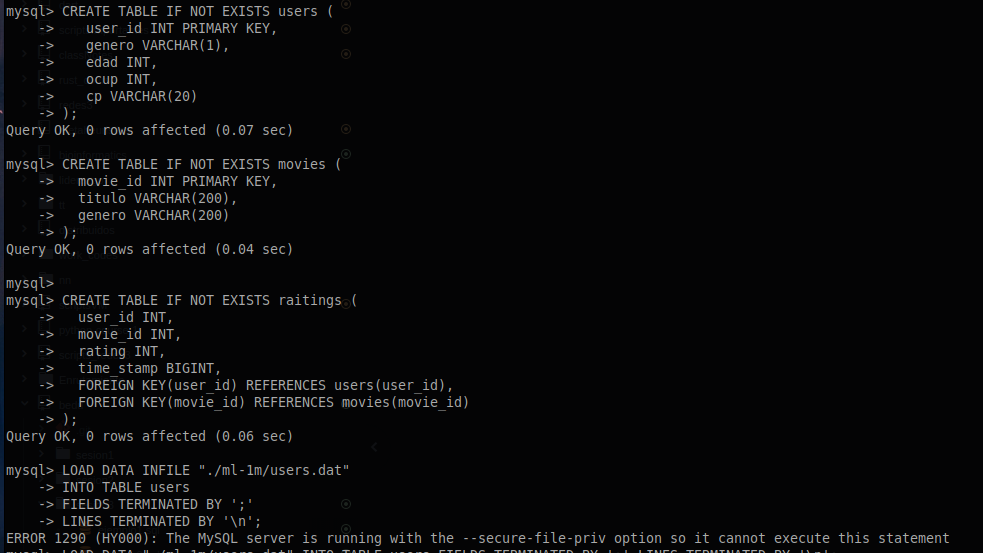
\includegraphics[scale=0.25]{imgs/1.png}\\
  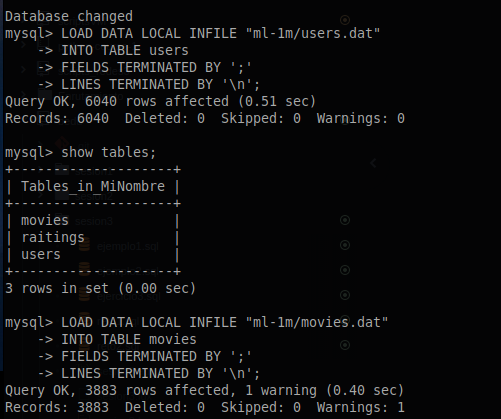
\includegraphics[scale=0.25]{imgs/2.png}\\
  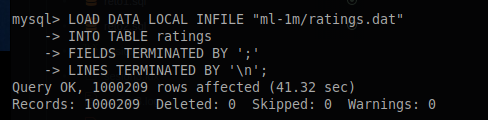
\includegraphics[scale=0.25]{imgs/3.png}\\
  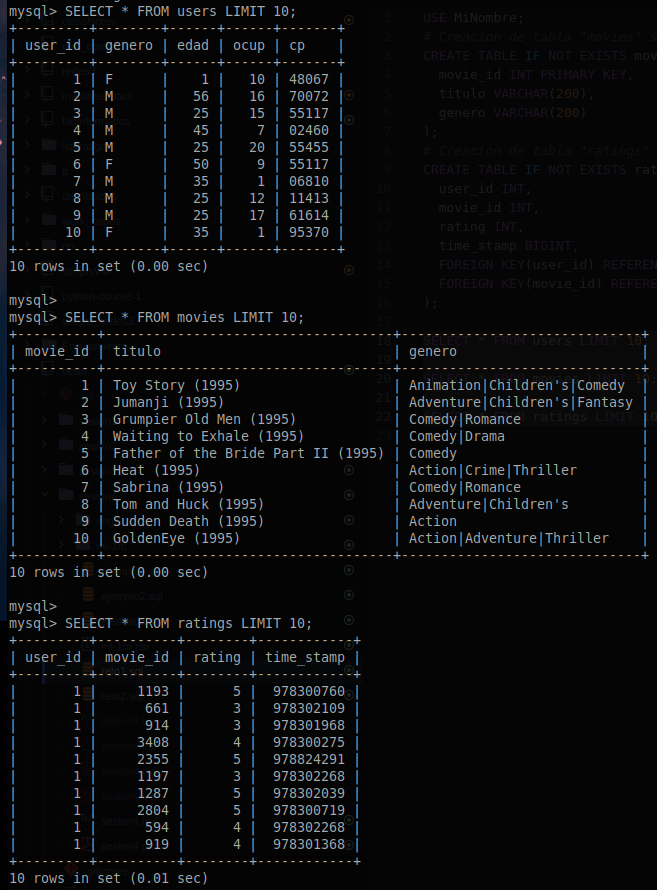
\includegraphics[scale=0.25]{imgs/4.png}\\
\end{center}

\section{MongoDB}
\begin{center}
  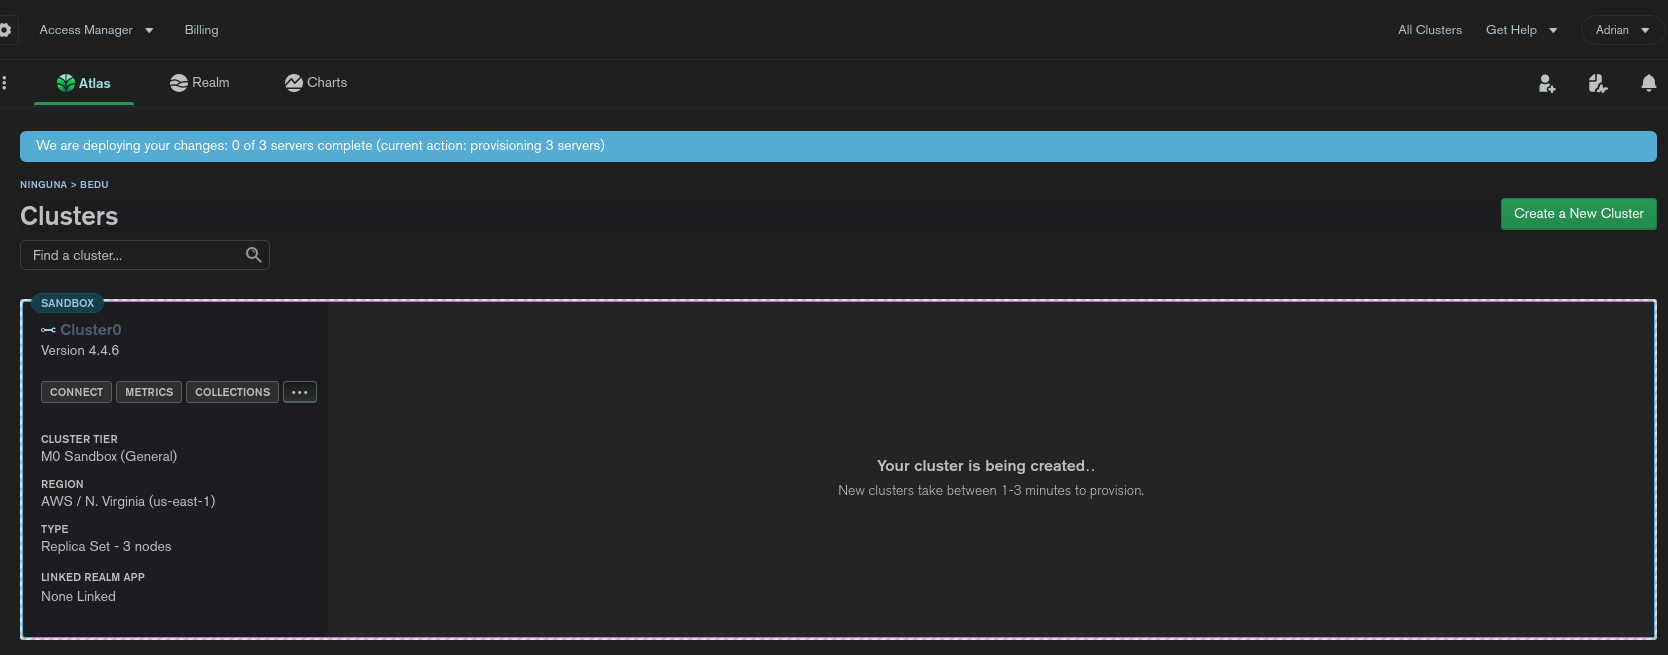
\includegraphics[scale=0.25]{imgs/5.png}\\
  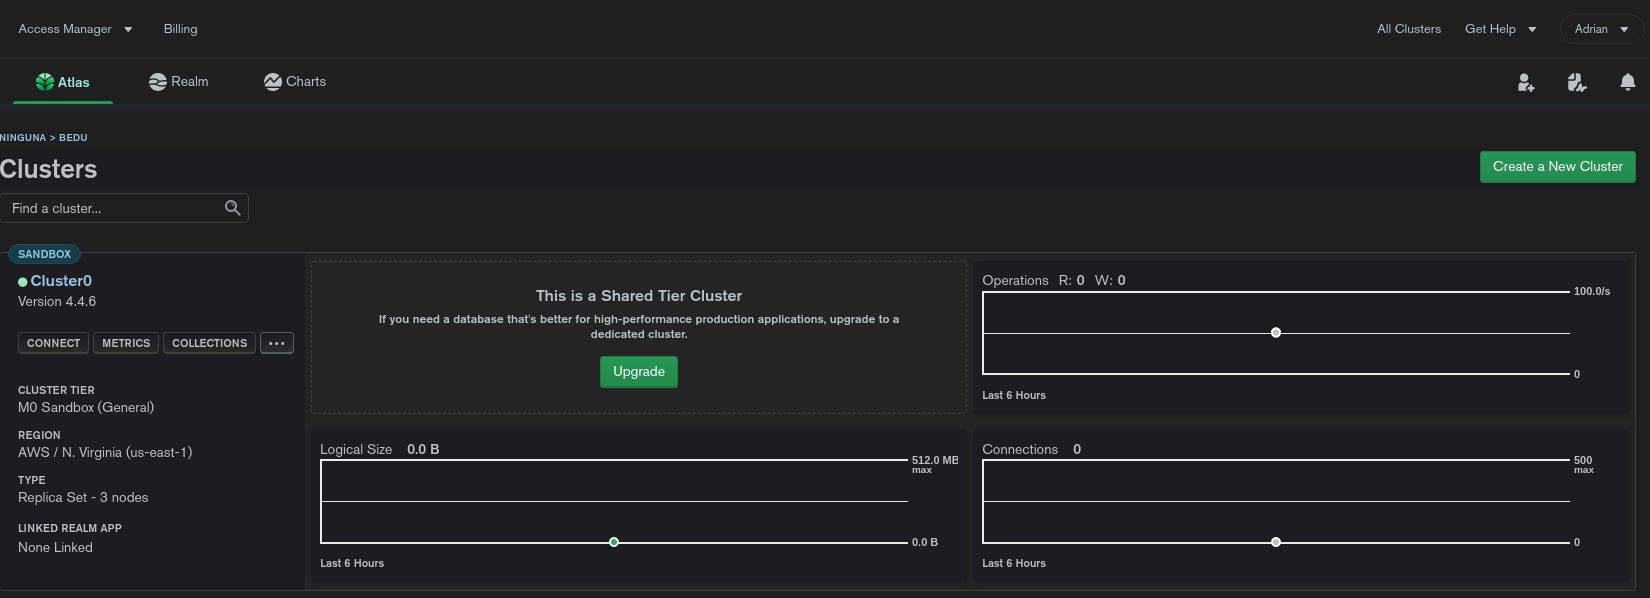
\includegraphics[scale=0.25]{imgs/6.png}\\
  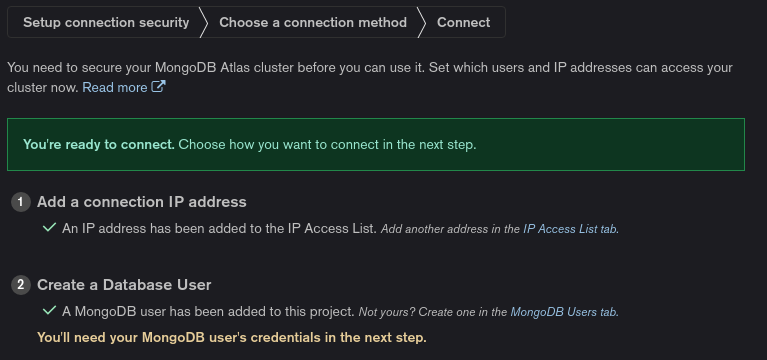
\includegraphics[scale=0.25]{imgs/7.png}\\
  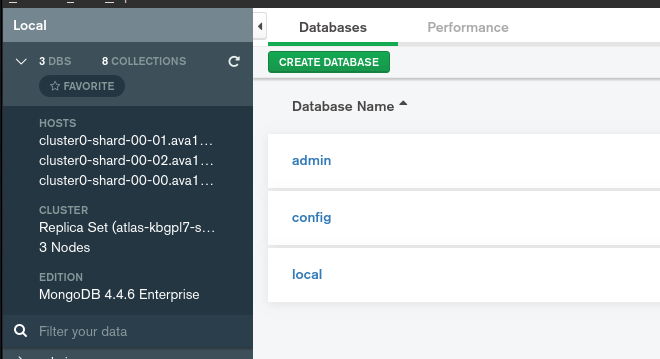
\includegraphics[scale=0.25]{imgs/8.png}\\
  \textit{Usuario y contraseña: introabd:introabd1234\\Más la creación del servidor de MongoDB}\\
  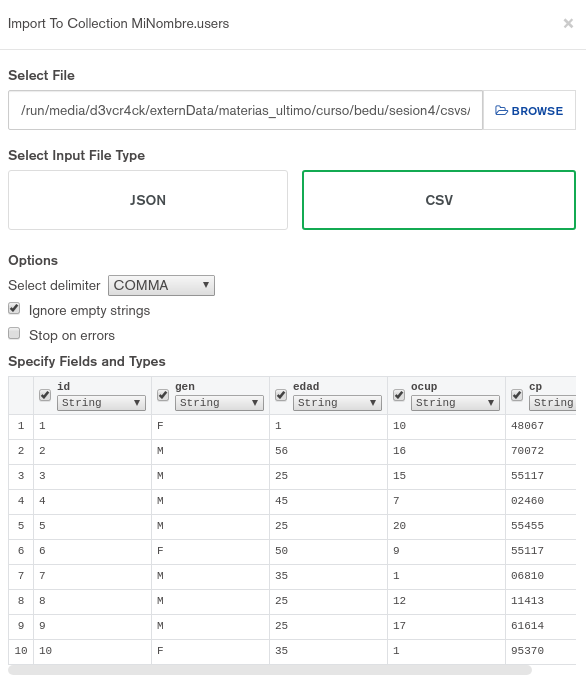
\includegraphics[scale=0.25]{imgs/9.png}\\
  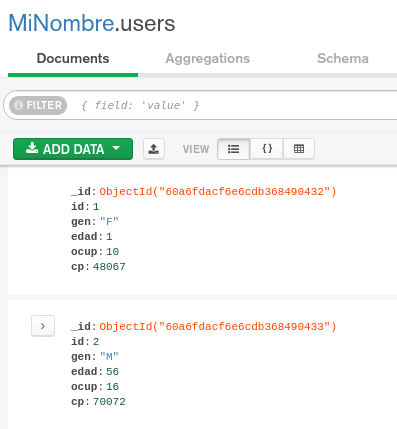
\includegraphics[scale=0.25]{imgs/10.png}\\
  \textit{Creación de colección users}\\
  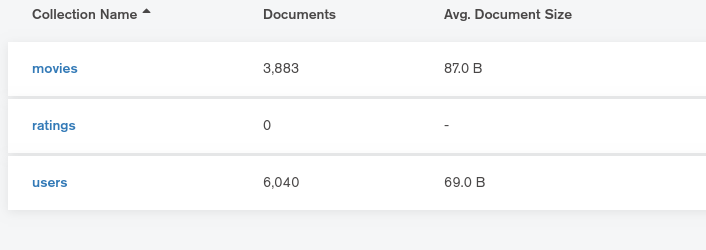
\includegraphics[scale=0.25]{imgs/11.png}\\
  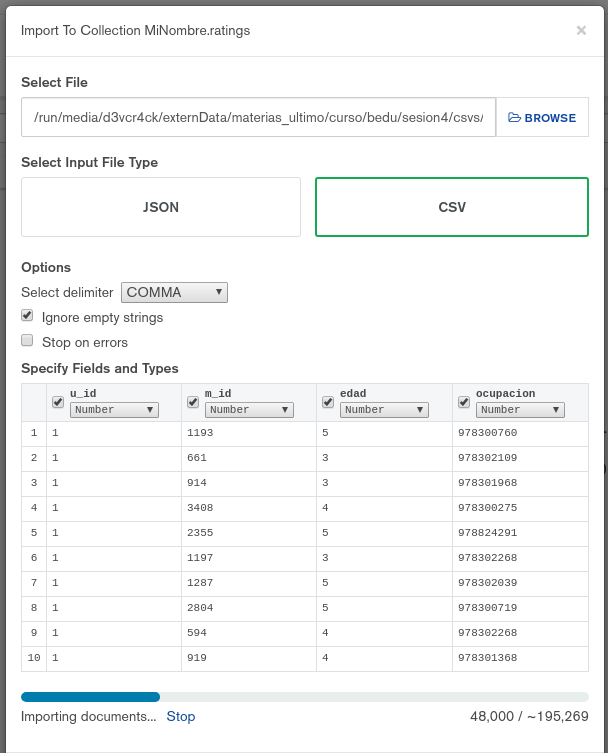
\includegraphics[scale=0.25]{imgs/12.png}\\
  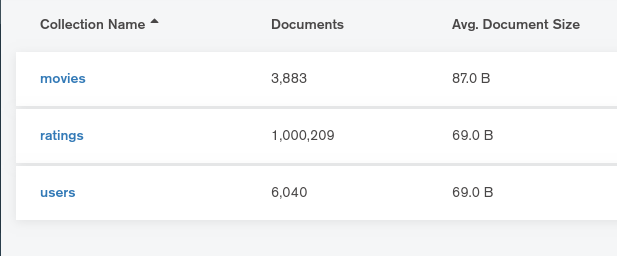
\includegraphics[scale=0.25]{imgs/13.png}\\
  \textit{Creación de colección movies y ratings con sus archivos csv respectivo}\\
  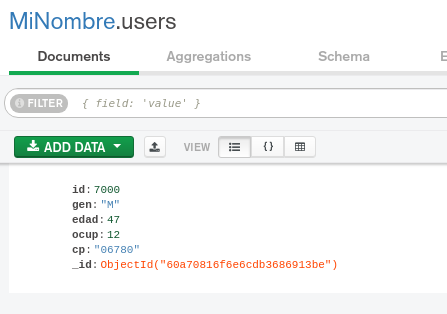
\includegraphics[scale=0.25]{imgs/14.png}\\
  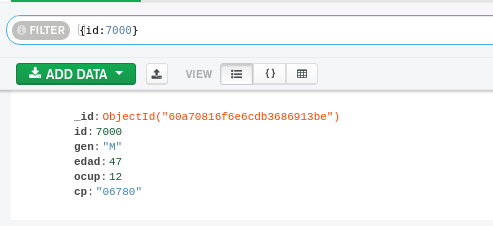
\includegraphics[scale=0.25]{imgs/15.png}\\
  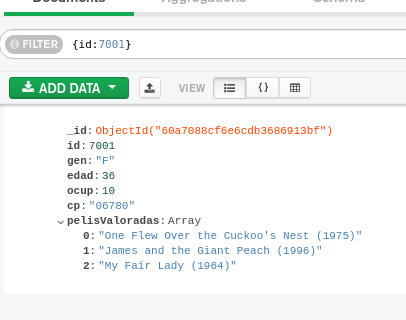
\includegraphics[scale=0.25]{imgs/16.png}\\
  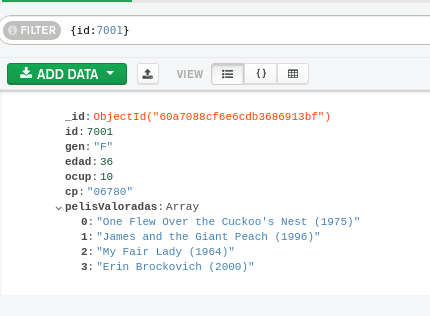
\includegraphics[scale=0.25]{imgs/17.png}\\
  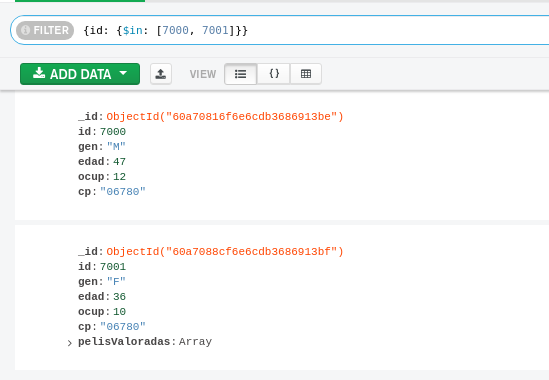
\includegraphics[scale=0.25]{imgs/18.png}\\
  \textit{Uso de la herramienta de MongoDB Compass para añadir, modificar, buscar información dentro de nuestra coleccion users}\clearpage
  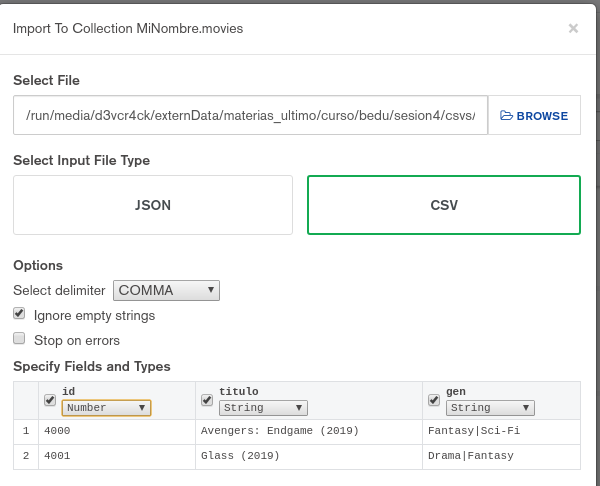
\includegraphics[scale=0.25]{imgs/19.png}\\
  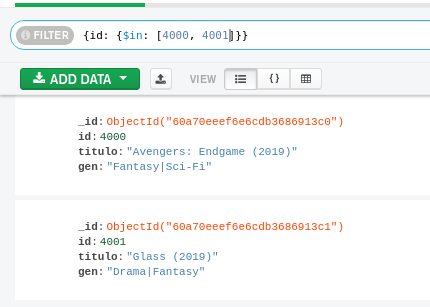
\includegraphics[scale=0.25]{imgs/20.png}\\
  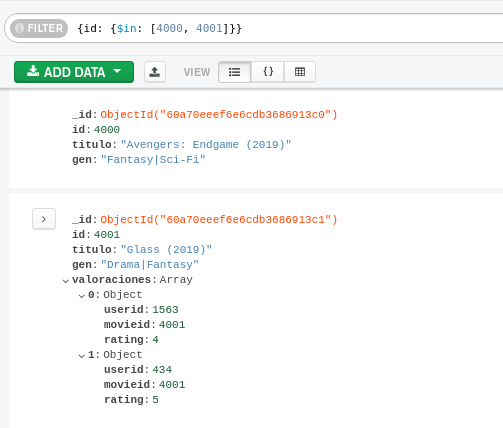
\includegraphics[scale=0.25]{imgs/21.png}\\
  \textit{Ejercicio de MongoDB en la colección movies}
\end{center}




\end{document}
